% Article template for Mathematics Magazine
% Revised 7/2002  Thanks for Greg St. George
\documentclass[12pt]{article}
\usepackage{amssymb}
\usepackage[ngerman]{babel}
\usepackage[utf8]{inputenc}
\usepackage{amsmath}
\usepackage{amsthm}
\usepackage{graphicx}
\renewcommand{\baselinestretch}{1.2}
%This is the command that spaces the manuscript for easy reading
\newtheorem{zeige}{Zeige}


%todo 
\usepackage[colorinlistoftodos,prependcaption,textsize=tiny]{todonotes}
\usepackage{xargs}                      % Use more than one optional parameter in a new commands
\newcommandx{\QUESTION}[2][1=]{\todo[linecolor=none,backgroundcolor=blue!15,bordercolor=none,#1]{\textbf{QUESTION: }#2}}



\begin{document}
%\thispagestyle{empty}
\begin{center}
\Large
% TITLE GOES HERE
Logik und Komplexität  \textsc{ Übung 7 }
\end{center}

\begin{flushright}
Denis Erfurt, 532437\\
HU Berlin \\

\vspace{2 mm}

\end{flushright}

\subsubsection*{Aufgabe 1)}

\paragraph{a)}

\begin{figure}[h]
 \centering
 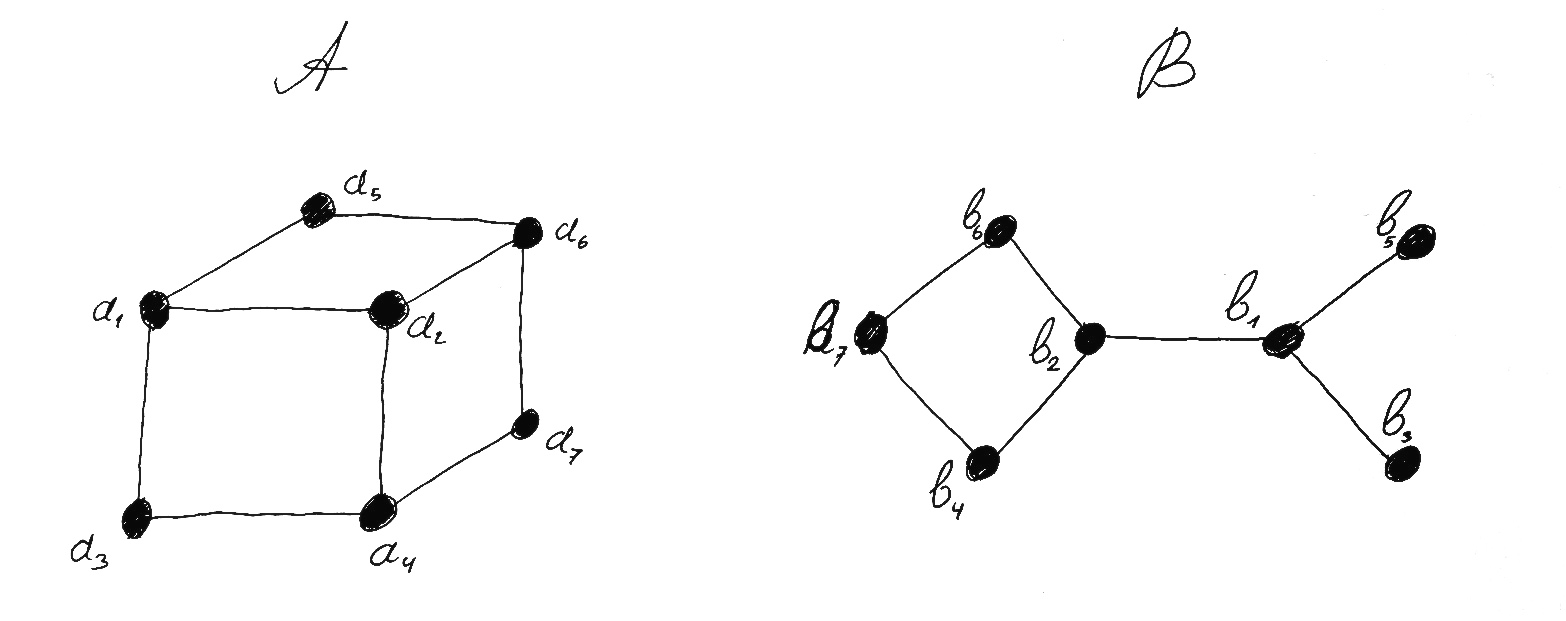
\includegraphics[width=0.8\textwidth]{struct.jpg}
 \caption{Strukturen}
 \label{struct}
\end{figure}

$b_1,b_2\in \mathfrak{B}$ so wie in Abbildung \ref{struct} angegeben.

\paragraph{b)}
Das größte m, so dass es $b_1, b_2\in B$ gibt mit $(A,a_1,a_2) \cong_m (B,b_1,b_2)$ ist $m=1$.

\textbf{zeige} dass $(I_j)_{j\leq 1}:(A,a_1,a_2) \cong_1 (B,b_1,b_2)$ ein Hin-und-Her-System ist.

\textbf{1)} $I_1 \neq \varnothing$

Sei $p = "\varnothing"$ die Abbildung, deren Definitionsberreich leer ist. $ I_1 = \{ p \}$
Sei $q: a_3 \mapsto b_3$. Klar ist, dass $q\supseteq p$
sowie $p,q\neq \varnothing$ und $q\in Part((A,a_1,a_2), (B,b_1,b_2))$

\textbf{2)} Wähle für jedes $a_i\in A$ ein $b_i\in B$ wie in Abbildung \ref{struct}. Klar ist: $ a_i \mapsto b_i \in Part((A,a_1,a_2), (B,b_1,b_2))$ sowie $a_i \mapsto b_i \supseteq p$

\textbf{3)} Wähle für jedes $b_i\in B$ ein $a_i\in A$ wie in Abbildung \ref{struct}. Klar ist: $ a_i \mapsto b_i \in Part((A,a_1,a_2), (B,b_1,b_2))$ sowie $a_i \mapsto b_i \supseteq p$

Somit ist $(I_j)_{j\leq 1}: (A,a_1,a_2) \cong_m (B,b_1,b_2)$ ein Hin-und-Her-System.

\paragraph{c)}
Angenommen $(I_j)_{j\leq 2}: (A,a_1,a_2) \cong_m (B,b_1,b_2)$ ist ein Hin-und-Her-System.
aus b) wissen wir, dass $p = a_3 \mapsto b_3 \in I_1$
Nach der "Hin-Eigenschaft" müsste für p und $a_4$ ein $q\in I_0$ geben, so dass $q\supseteq p$ und $a_4 \in Def(q)$.

Jedoch ist für jedes $b_i\in B: a_3,a_4 \mapsto b_3,b_i \notin Part((A,a_1,a_2), (B,b_1,b_2))$ 

Somit folgt, dass $(I_j)_{j\leq 2}: (A,a_1,a_2) \cong_m (B,b_1,b_2)$ kein Hin-und-Her-System ist. 


\subsubsection*{Aufgabe 2)}
Sei $GG\subseteq UGraph$ die Klasse der Strukturen, bei denen jeder Knoten 
einen Geraden Grad besitzt. 

zeige $GG$ ist nicht EMSO-definierbar in $UGraph$.

Laut dem Satz von Ajtai und Fagin genügt es zu zeigen, dass Duplicator eine 
Gewinnstrategie im (l,m)-Ajtai-Fagin-Spiel besitzt.

\textbf{Phase 1.} Duplicator wählt einen vollständigen-Graphen $\mathfrak{A} = K_{2^{l+m}+1}$.

\textbf{Beobachtung:} für einen vollständigen-Graphen gilt:
  \[ \text{n ist ungerade} \Leftrightarrow K_n \in GG \] 
  
Spoiler wählt hiernach die Mengen $X_1^\mathfrak{A}, ..., X_l^\mathfrak{A} 
\subseteq V$

Sei $c^\mathfrak{A}(a) := \{ X_i^\mathfrak{A} : a\in X_i^\mathfrak{A} \}$ die
Farbe eines Knotens $a$. 

Für jede Farbe $f\subseteq \{ X_1^\mathfrak{A}, ..., X_l^\mathfrak{A} \}$ sei

\[ M_f^\mathfrak{A} := \{ a \in A : c^\mathfrak{A}(a) = f \} \] 

\textbf{zeige: } nach l Mengen exestiert exestiert ein $M_f^\mathfrak{A}$ so 
dass $|M_f^\mathfrak{A}| \geq 2^m$

  Beweis durch vollständige Induktion: 
  
  \textbf{Induktionsannahme:} nach der i-ten Menge $X_i^\mathfrak{A}$ exestiert
  ein $f$ mit $|M_f^\mathfrak{A}| \geq 2^{l-i+m}$

  \textbf{Induktionsanfang:} $i=0$ Wir wissen dass $|A| = 2^{l+m}$. Für $f=\{\}$
  ist $M_f^\mathfrak{A} = A \Rightarrow |M_f^\mathfrak{A}|\geq 2^{l+m}$

  \textbf{Induktionsschritt:} $i \rightarrow i+1$
  Nach \textbf{IA} exestiert ein $f$ mit $|M_f^\mathfrak{A}|\geq 2^{l-i+m}$
  Spoiler wählt ein $X_{i+1}^\mathfrak{A}$.

  Sei $f' := f \cup \{X_{i+1}^\mathfrak{A}\}$

  Nach \textbf{IA} wissen wir:
  \[ |M_{f'}^\mathfrak{A}| + |M_f^\mathfrak{A}| \geq 2^{l-i+m} \] 

  Falls $|M_{f'}^\mathfrak{A}| < 2^{l-(i+1)+m}$, dann folgt daraus 
  $|M_f^\mathfrak{A}|\geq 2^{m-(i+1)+m}$

  Falls $|M_f^\mathfrak{A}| < 2^{l-(i+1)+m}$, dann folgt daraus 
  $|M_{f'}^\mathfrak{A}|\geq 2^{m-(i+1)+m}$

  \textbf{Indunktionsschluss:} Nach l Mengen exestiert eine Farbe f mit 
  $|M_f^\mathfrak{A}|\geq 2^{m}$
  
\textbf{Phase 2.} Duplicator wählt $\mathfrak{B} = K_{2^{l+m}+2}$. Nach Beobachtung
ist $\mathfrak{B}\in UGraph \setminus GG$
Weiter wählt Duplicator die Mengen $X_1^\mathfrak{B}, ..., X_l^\mathfrak{B}$ so, 
dass für jede Farbe $f$ gilt:
\begin{equation}
  |M_f^\mathfrak{B}|=|M_f^\mathfrak{A}|\text{ oder } |M_f^\mathfrak{B}|,|M_f^\mathfrak{A}|
  \geq 2^m \label{eq}
\end{equation}
Intuitiv färbt Duplicator den neuen Knoten mit der in $\mathfrak{A}$ häufigsten Farbe.

\textbf{Phase 3.} Betrachte das EF-Spiel auf $\mathfrak{A}' := (\mathfrak{A}, 
X_1^\mathfrak{A}, ... , X_l^\mathfrak{A})$ und $\mathfrak{B}' := (\mathfrak{B}, 
X_1^\mathfrak{B}, ... , X_l^\mathfrak{B})$

Für jede Wahl $a_i\in A$ von Spoiler kann Dup wegen (\ref{eq}) ein $b_i\in B$ wählen,
so dass $c(a)^\mathfrak{A} = c(b)^\mathfrak{B}$:
Falls $|M_f^\mathfrak{B}|=|M_f^\mathfrak{A}|$ so hat Duplicator eine Gewinnstrategie, 
in dem er Spoilers züge Kopiert. Falls $|M_f^\mathfrak{B}|,|M_f^\mathfrak{A}|
\geq 2^m $ so besitzt Duplicator eine Gewinnstrategie, indem er ein neues Element wählt,
falls Spoiler ein neues Element mit dieser Farbe gewählt hat. Andernfalls falls Spoiler
ein in Runde i gewähltes Element wählt, so wählt Duplicator in Runde i gewählte Element
der anderen Struktur. 
Analog für Spoilers wahl aus $\mathfrak{B}$.

Somit ist gezeigt das Duplicator eine Gewinnstrategie im (l,m)-Ajtai-Fagin-Spiel
besitzt. Somit ist nach Satz 3.44 $GG$ nicht EMSO-definierbar in $UGraph$. \qed

\subsubsection*{Aufgabe 3)}

Angelehnt an Beispiel 4.6 c)\\
Sei k:=4. Zur Erinnerung: $EA_k = EA_{2k,k}$\\
Für jeden Graphen $G=(V,E)$ mit $G \models EA_k$ und $|V| \geq 2k = 4$ gilt gemäß Beob. 4.3:\\
$G \models EA_{l,m}\ f.a.\ l\geq 1, m\geq 0\ mit\ m\leq l \leq k$\\
Aus $G \models EA_{1,1}$ und $|V| > 1$ folgt: Es gibt Knoten a und b, s.d. diese Verbunden sind.\\
Weiter folgt aus $G \models EA_{2,2}$ mit $S:={a,b}=T$, dass es einen Knoten c nicht aus der Menge gibt, s.d. c zu a und b verbunden ist. Dies ist ein Dreieck, also der vollständige Graph $K_3$.   \\
- $G \models EA_{3,3}$ mit $S:=\{a,b,c\}=T$, es gibt d, s.d. d zu a,b,c verbunden ist. Dies bildet $K_4$. \\
- $G \models EA_{4,4}$ mit $S:=\{a,b,c,d\}=T$, es gibt e, s.d. e zu a,b,c,d verbunden ist. Dies bildet $K_5$. \\

Die Menge aller nicht-planaren Graphen ist größer/gleich der Menge derer, die einen $K_5$-Teilgraphen haben.
Somit gilt für die planaren Graphen die Gegenwahrscheinlichkeit:\\
$\mu_n(NP | UG) \geq  \mu_n(EA_4 | UG) \rightarrow_{n \rightarrow \infty} 1$\\
$\mu_n(P | UG) = 1 - \mu_n(NP | UG) = 0$
\begin{flushright}
$\square$
\end{flushright}

\subsubsection*{Aufgabe 4)}
\paragraph{a)}
Sei $\leq(a,b):=$'a steht vor b in w'.\\
Für jedes $l\in \mathbb{N}\ seien\ x_1 .. x_{l+1}$ paarweise verschieden und sei\\
$\Delta^{\sigma_{\{a,b\}}}_{l+1} := \{ \leq(a,x_{l+1}) : a \in \{x_1, .., x_{l+1}\} \}$\\
(Teile das Wort in zwei Partitionen, Buchstaben kleiner bzw. größer $x_{l+1}$)\\
Für $F \subseteq \Delta^{\sigma_{\{a,b\}}}_{l+1}$ sei $\bar F:=\Delta^{\sigma_{\{a,b\}}}_{l+1} \backslash F$\\
$EA_{l,F}:=\forall x_1 .. x_{l+1} (\bigwedge\limits_{1 \leq i < j \leq l} x_i \neq x_j \rightarrow$ 
$\exists x_{l+1}(\bigwedge\limits_{i=1}^l x_{l+1} \neq x_i \land \bigwedge\limits_{\phi \in F} \phi \land \bigwedge\limits_{\psi \in \bar F} \neg \psi))$\\
Bws: $\xi :=  \{ EA_{l,F} : 0 \leq l \leq k = $'Wortlänge'$\}$\\
Beobachte: $\xi$ ist endlich.\\
$\eta := \bigwedge\limits_{\phi \in F} \phi$\\
Seien ALL alle Wortstrukturen.\\
Sollte es eine $\sigma$-Struktur geben, die $\eta \ und\ \psi$ erfüllt, dann gilt f.a. n$\geq$1:\\
$\mu_n(\phi | ALL) \geq \mu_n (\eta | ALL) \rightarrow 1$\\
Ansonsten: $\mu_n(\neg \phi | ALL) \geq \mu_n (\eta | ALL) \rightarrow 1$ und somit $\mu_n(\phi | ALL) = 0$
\begin{flushright}
$\square$
\end{flushright}
\paragraph{b)}
Aus Beispiel 2.10 wissen wir dass es ein EMSO-Satz $\phi_{even}$ gibt, der genau die Strukturen Beschreibt deren Universum gerade Kardinalität haben. Außerdem wissen wir aus Beispiel 4.1 a) dass $\mu( EVEN | ALL ) = undefined$ ist. Demnach besitzt $MSO[\leq]$ kein 0-1-Gesetz bzgl. der Klasse aller endlichen linearen Ordnungen.
\paragraph{c)}
analog zu a)
\paragraph{d)}
Sei S die Klasse der Strukturen, die einen vollständigen Graphen beinhalten, falls das Universum gerade ist. Außerdem besitz S die Graphen ohne Verbindungen falls das universum ungerade ist. 
\[ S:=\{(V,E):|V|\text{ ist gerade und } E=V^2\} \cup \{(V,E):|V|\text{ ist ungerade und } E=\emptyset\} \] 
Daraus folgt analog zu Beispiel 4.1 a):
$$\phi:=\exists x\exists y E(x,y)\Rightarrow  \mu_n(\phi|S) = undefined $$

Somit beistzt $FO[E]$ kein 0-1-Gesetz bezüglich S. 

\end{document}
